\documentclass{beamer}
% theme général du diaporama
\usetheme{Boadilla}
%paquets pour le français
\usepackage[T1]{fontenc}
\usepackage[utf8]{inputenc}
%package pour les images
\usepackage{graphicx}

\subtitle{}
\title{5G: En marche vers une revolution?}
\institute[Paris 8]{Paris VIII}
\author{Chaolei CAI}
\date{\today}
%modifie le fond de la presentation
\setbeamercolor{background canvas}{bg = white}
%\setbeamercovered{transparent}
%\usecolortheme[named=gray]{structure}


\begin{document}

    \frame{\titlepage}
    \tableofcontents

    \section{Un peu d'histoire}

    \begin{frame}
        \frametitle{Réseau Radiocom 2000}
        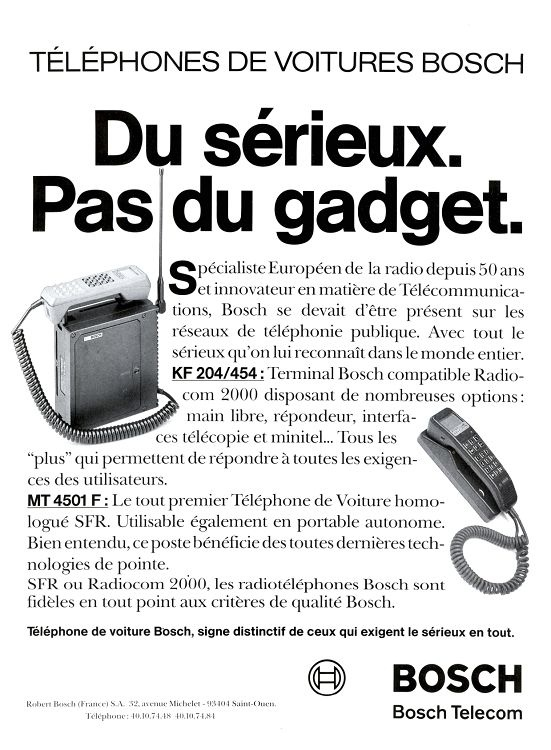
\includegraphics[width=0.70\textwidth,height=0.9\textheight]{img/bosch.jpg}
    \end{frame}


    \begin{frame}
        \frametitle{Global System for Mobile Communications}
        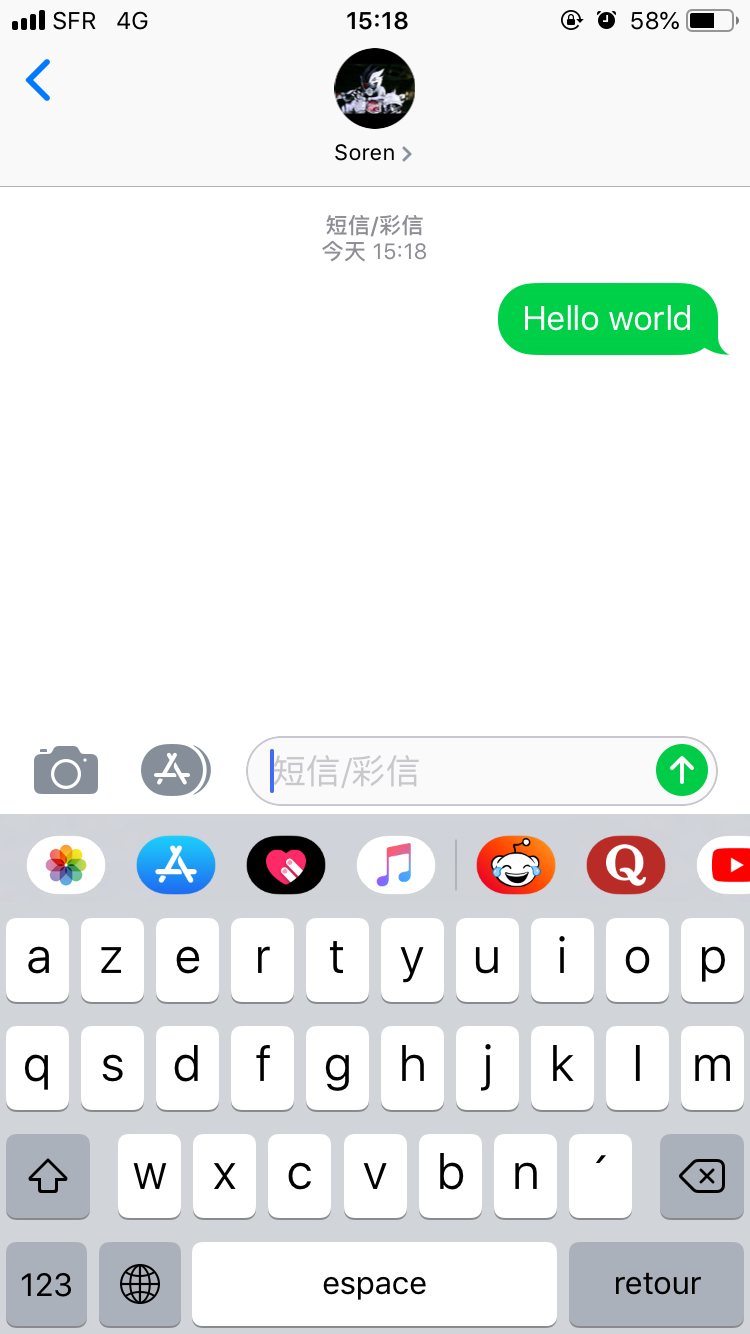
\includegraphics[width=0.5\textwidth,height=0.9\textheight]{img/sms.jpg}
        9,05 kbit/s
    \end{frame}

    \begin{frame}
        \frametitle{Universal Mobile Telecommunications System}
        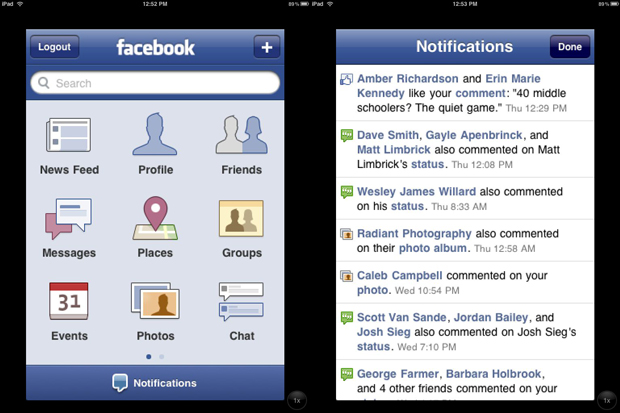
\includegraphics[width=\linewidth,height=0.9\textheight]{img/facebook.jpg}
        1,9 Mbit/s
    \end{frame}

    \begin{frame}
        \frametitle{Long Term Evolution Advanced}
        
\includegraphics[width=\linewidth,height=0.9\textheight]{img/fb-tw.jpg}
        1 Gbit/s
    \end{frame}

    \section{La 5G}
    \begin{frame}
        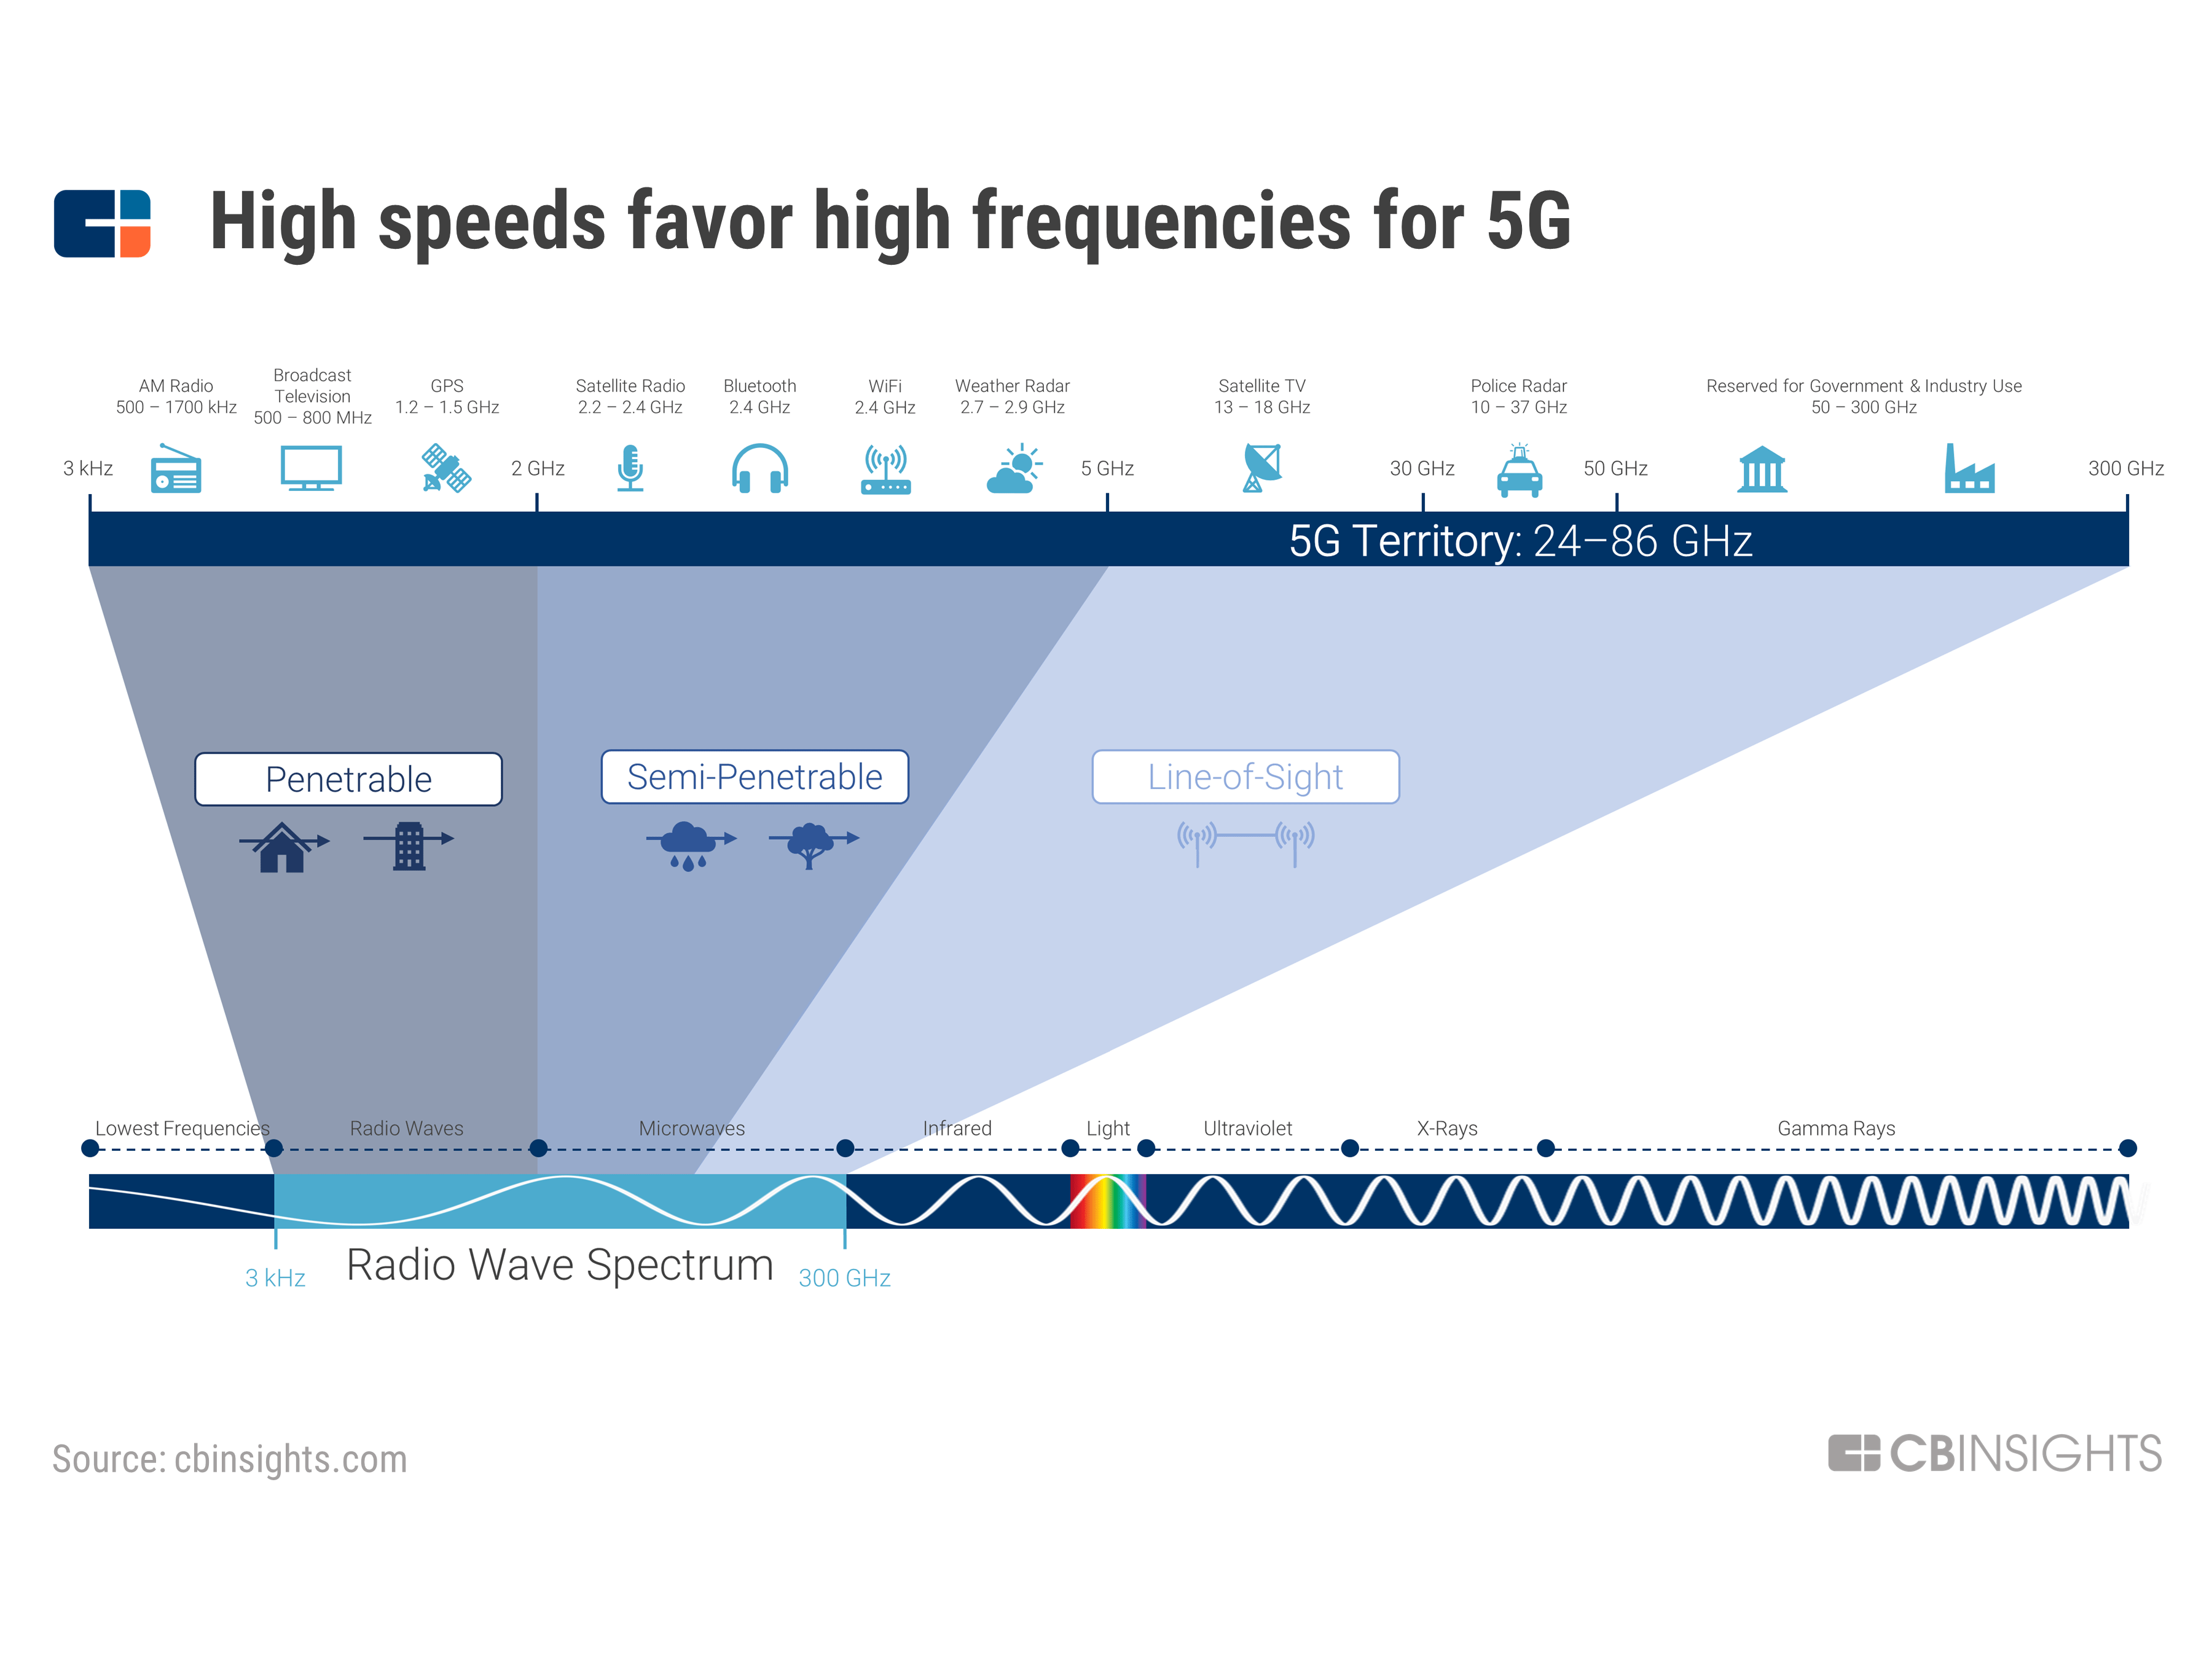
\includegraphics[width=\linewidth]{img/5G-Spectrum.png}
    \end{frame}

    \begin{frame}
        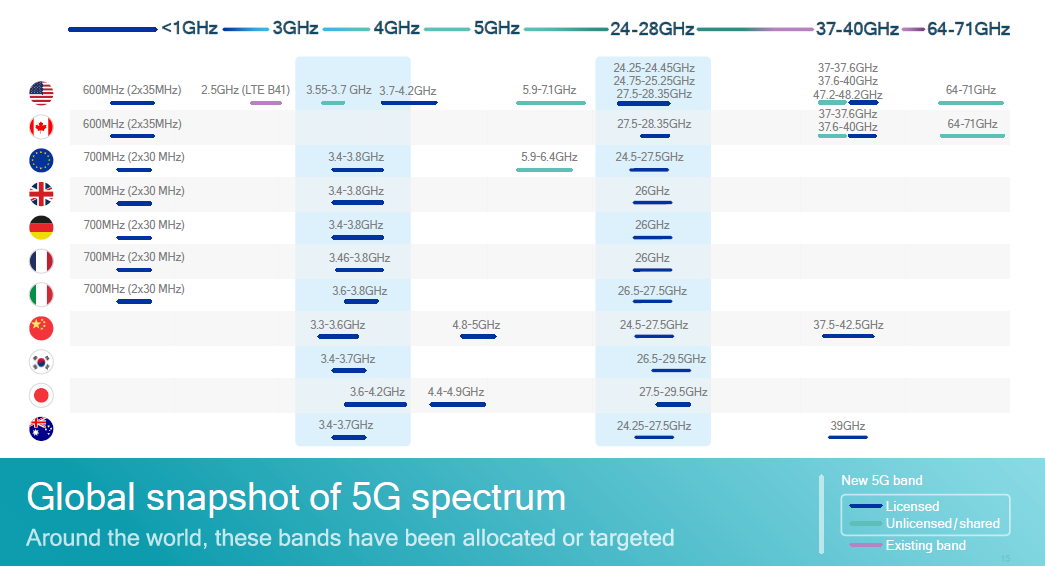
\includegraphics[width=\linewidth]{img/5Gbands.PNG}
    \end{frame}

    \begin{frame}
        \frametitle{Small Cells}
        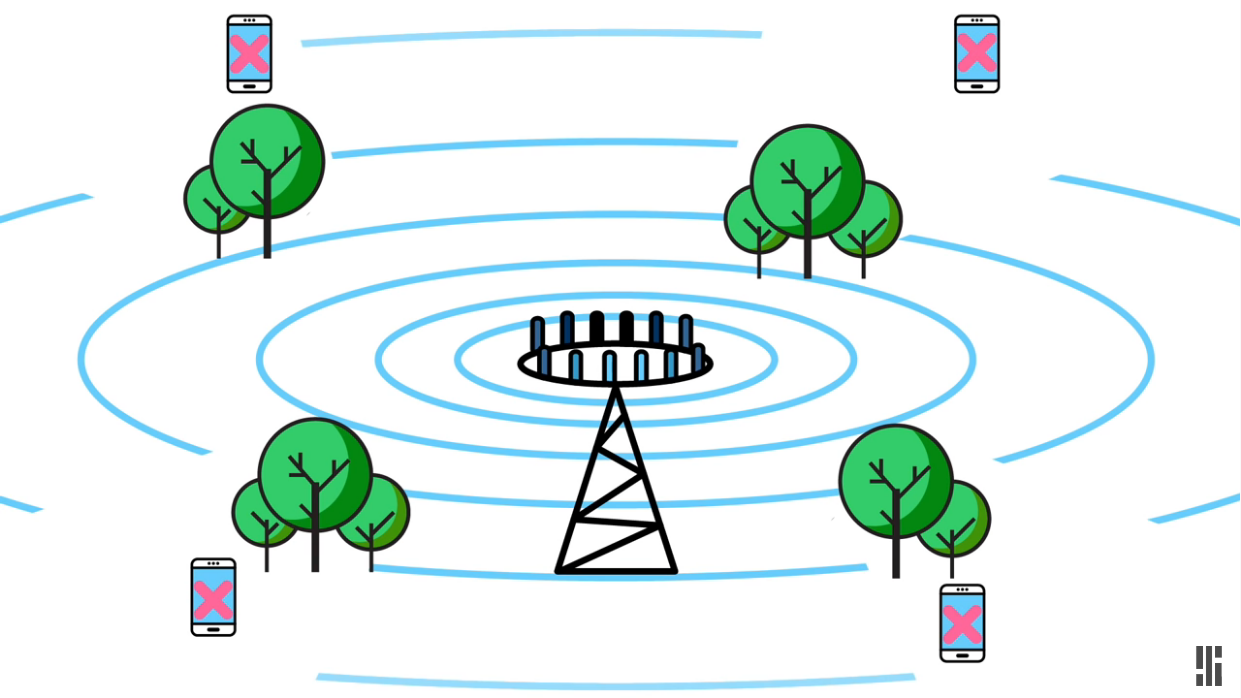
\includegraphics[width=\linewidth]{img/SmallCell1.png}
    \end{frame}

    \begin{frame}
        \frametitle{Small Cells}
        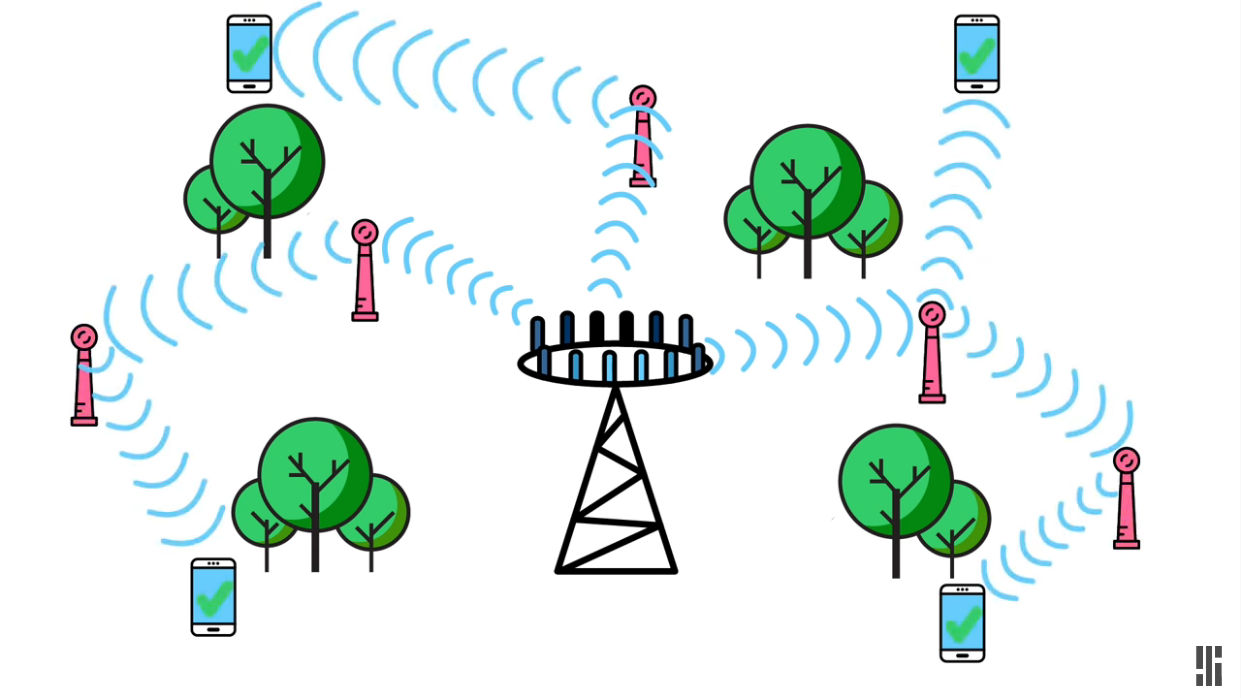
\includegraphics[width=\linewidth]{img/SmallCell2.png}
    \end{frame}

    \begin{frame}
        \frametitle{Massive MIMO(Multiple Input Multiple Output)}
        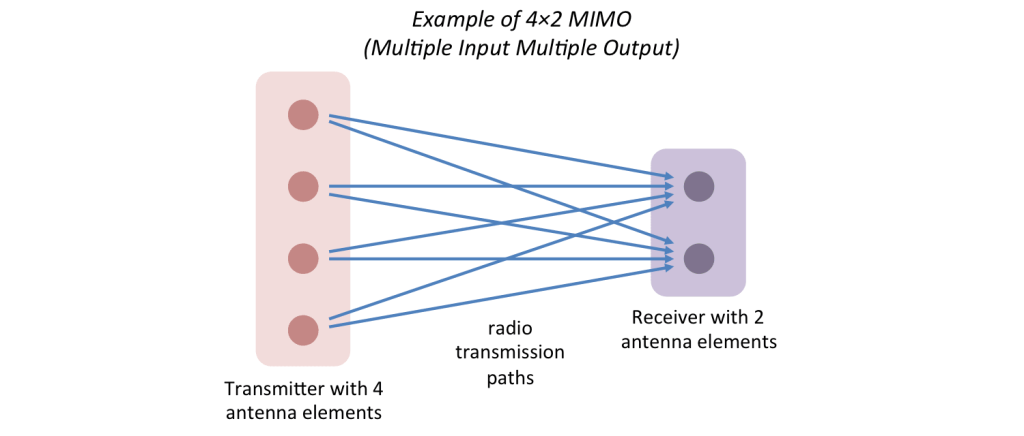
\includegraphics[width=\linewidth]{img/MIMO.png}
    \end{frame}

    \begin{frame}
        \frametitle{Massive MIMO(Multiple Input Multiple Output)}
        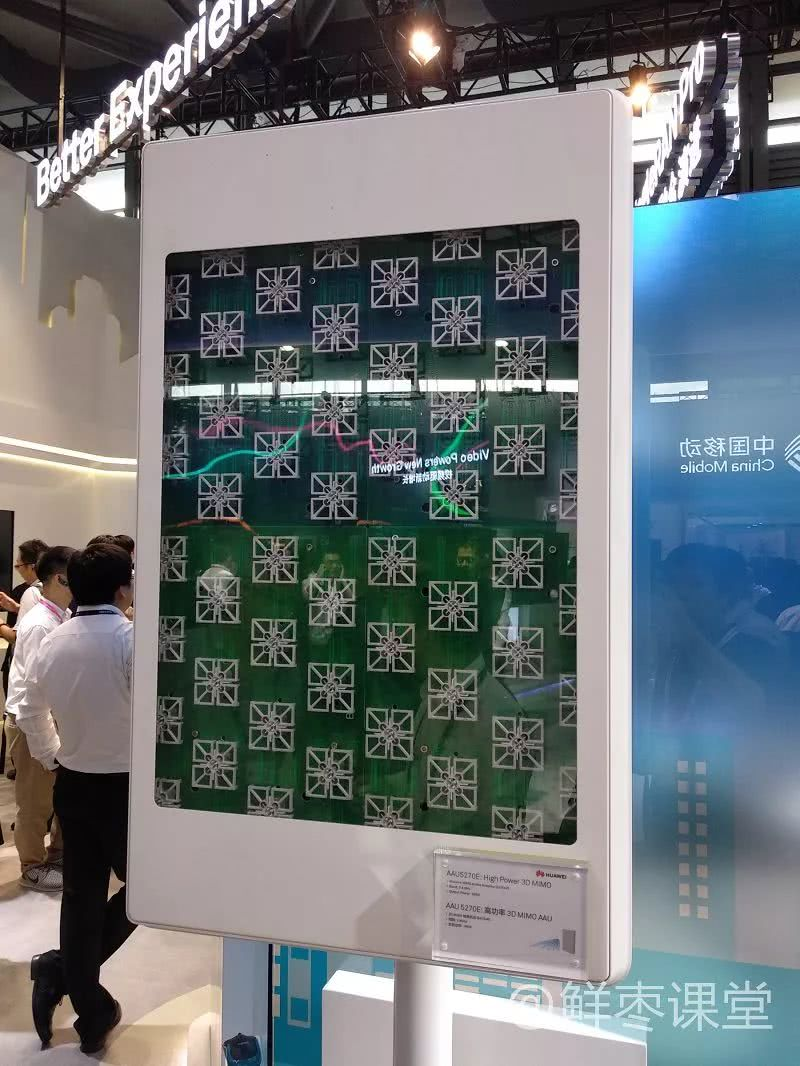
\includegraphics[height=0.9\textheight]{img/huawei.jpg}
    \end{frame}

    \begin{frame}
        \frametitle{BeamForming}
        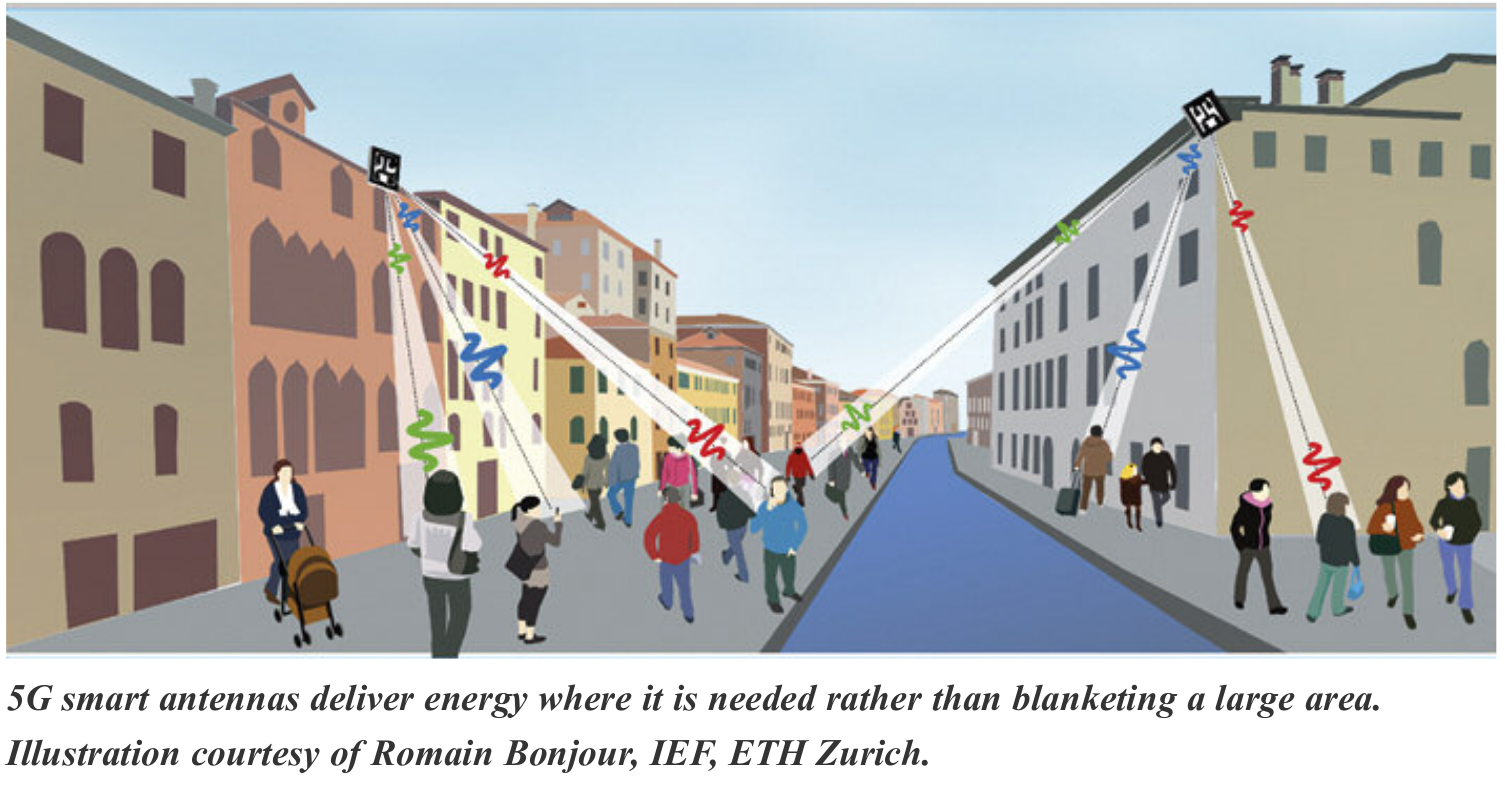
\includegraphics[width=\linewidth]{img/BeamForming.png}
    \end{frame}

    \begin{frame}
        \frametitle{Full Duplex}
        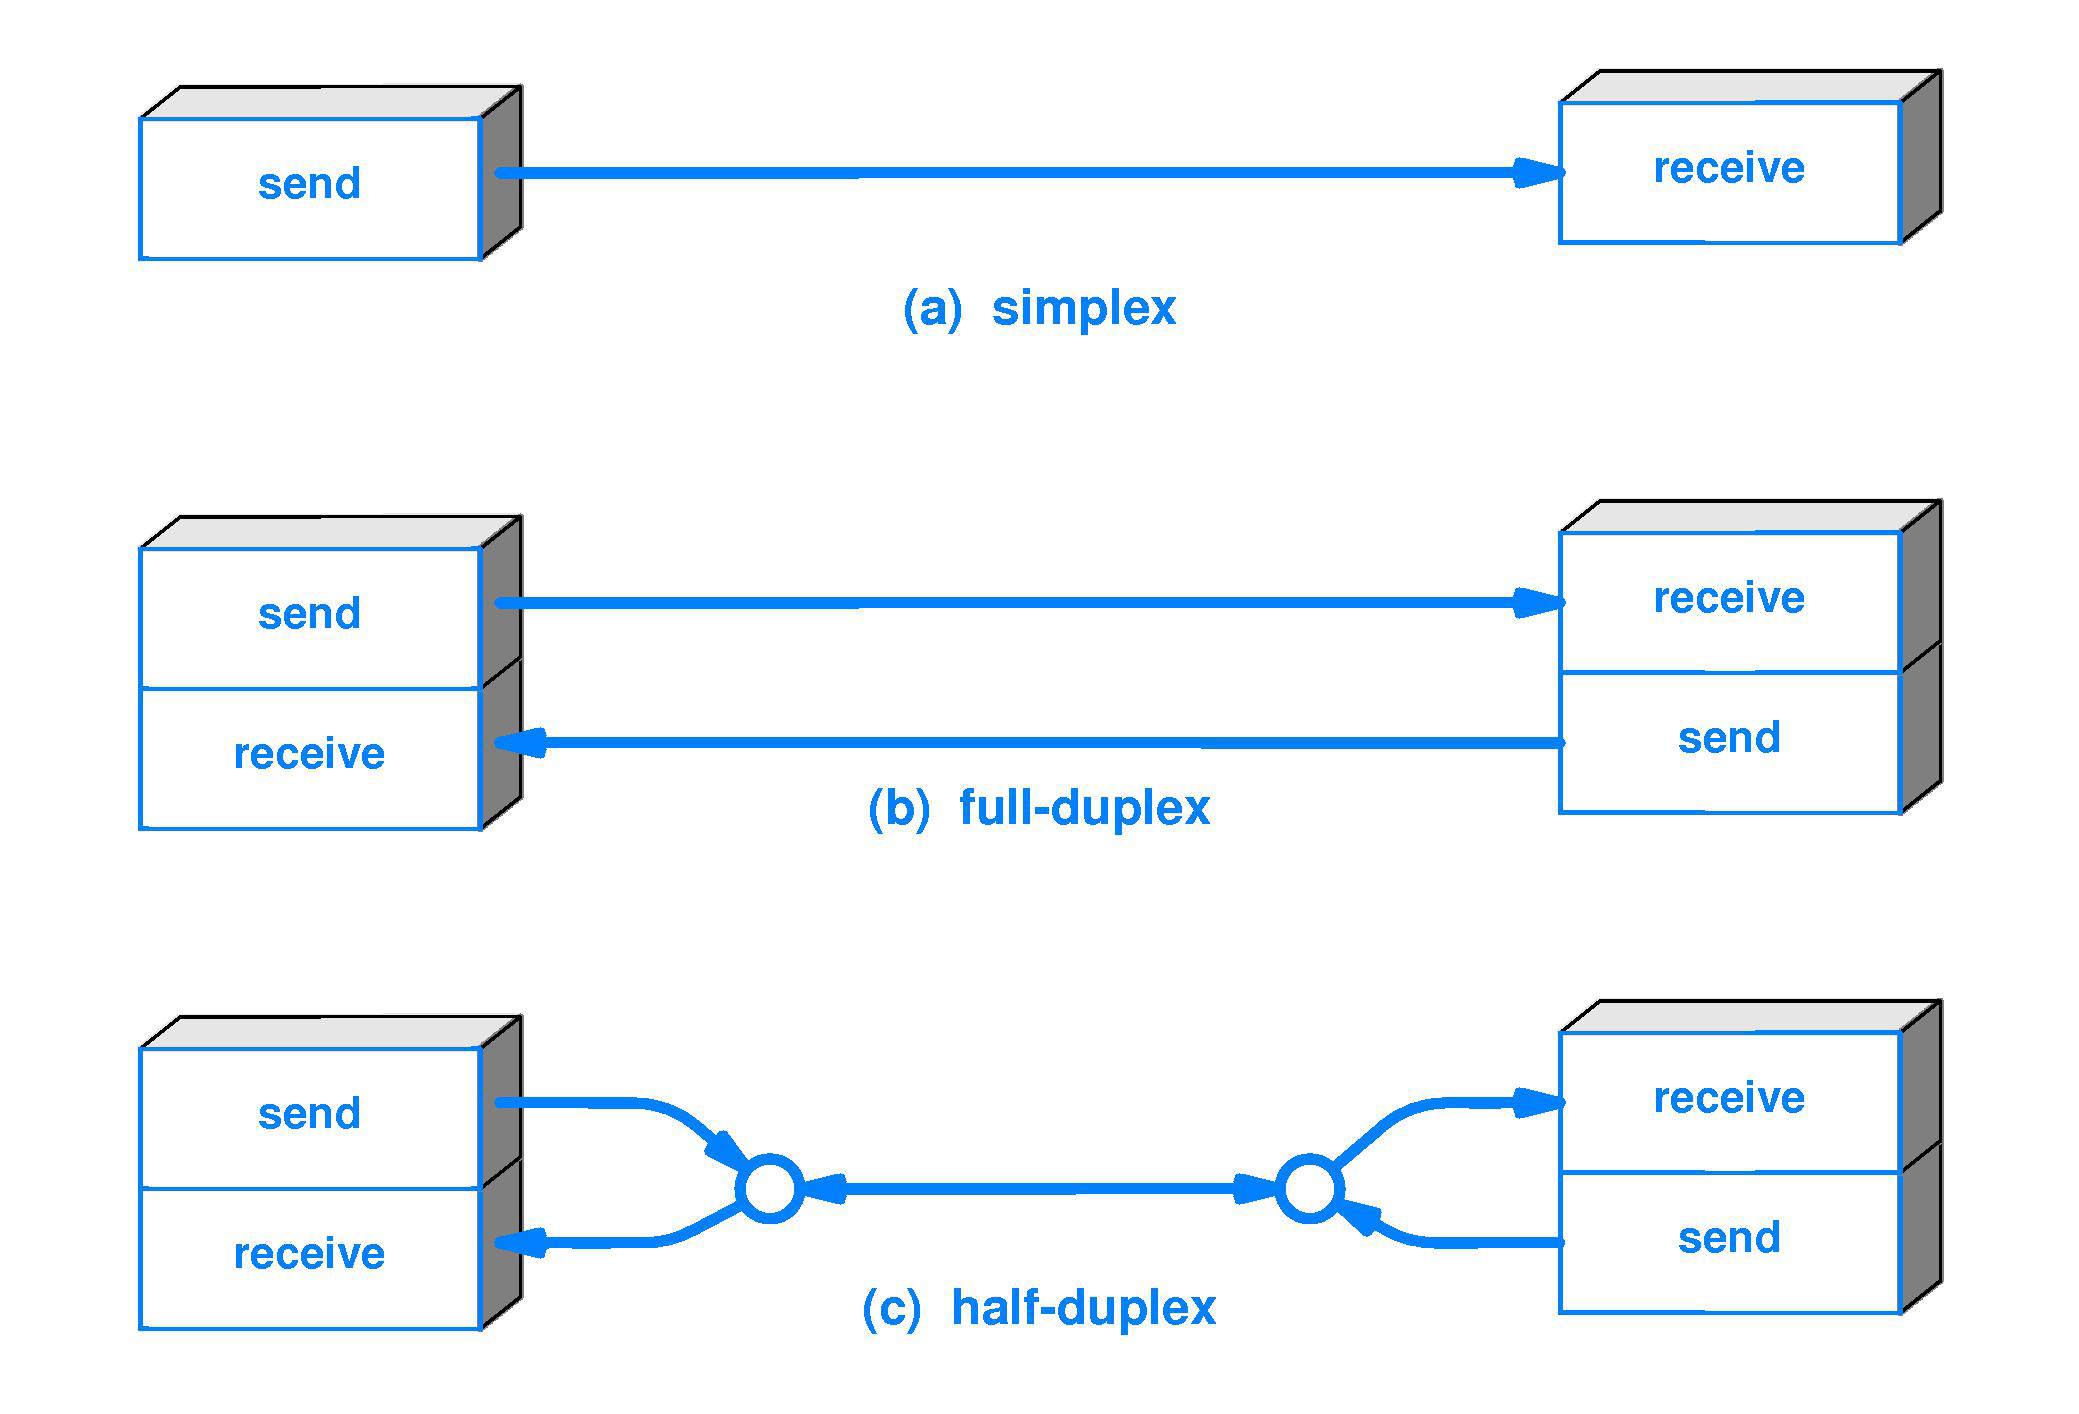
\includegraphics[width=\linewidth]{img/full-duplex.jpg}
    \end{frame}

    \begin{frame}
        \frametitle{Un risque pour la santé}
        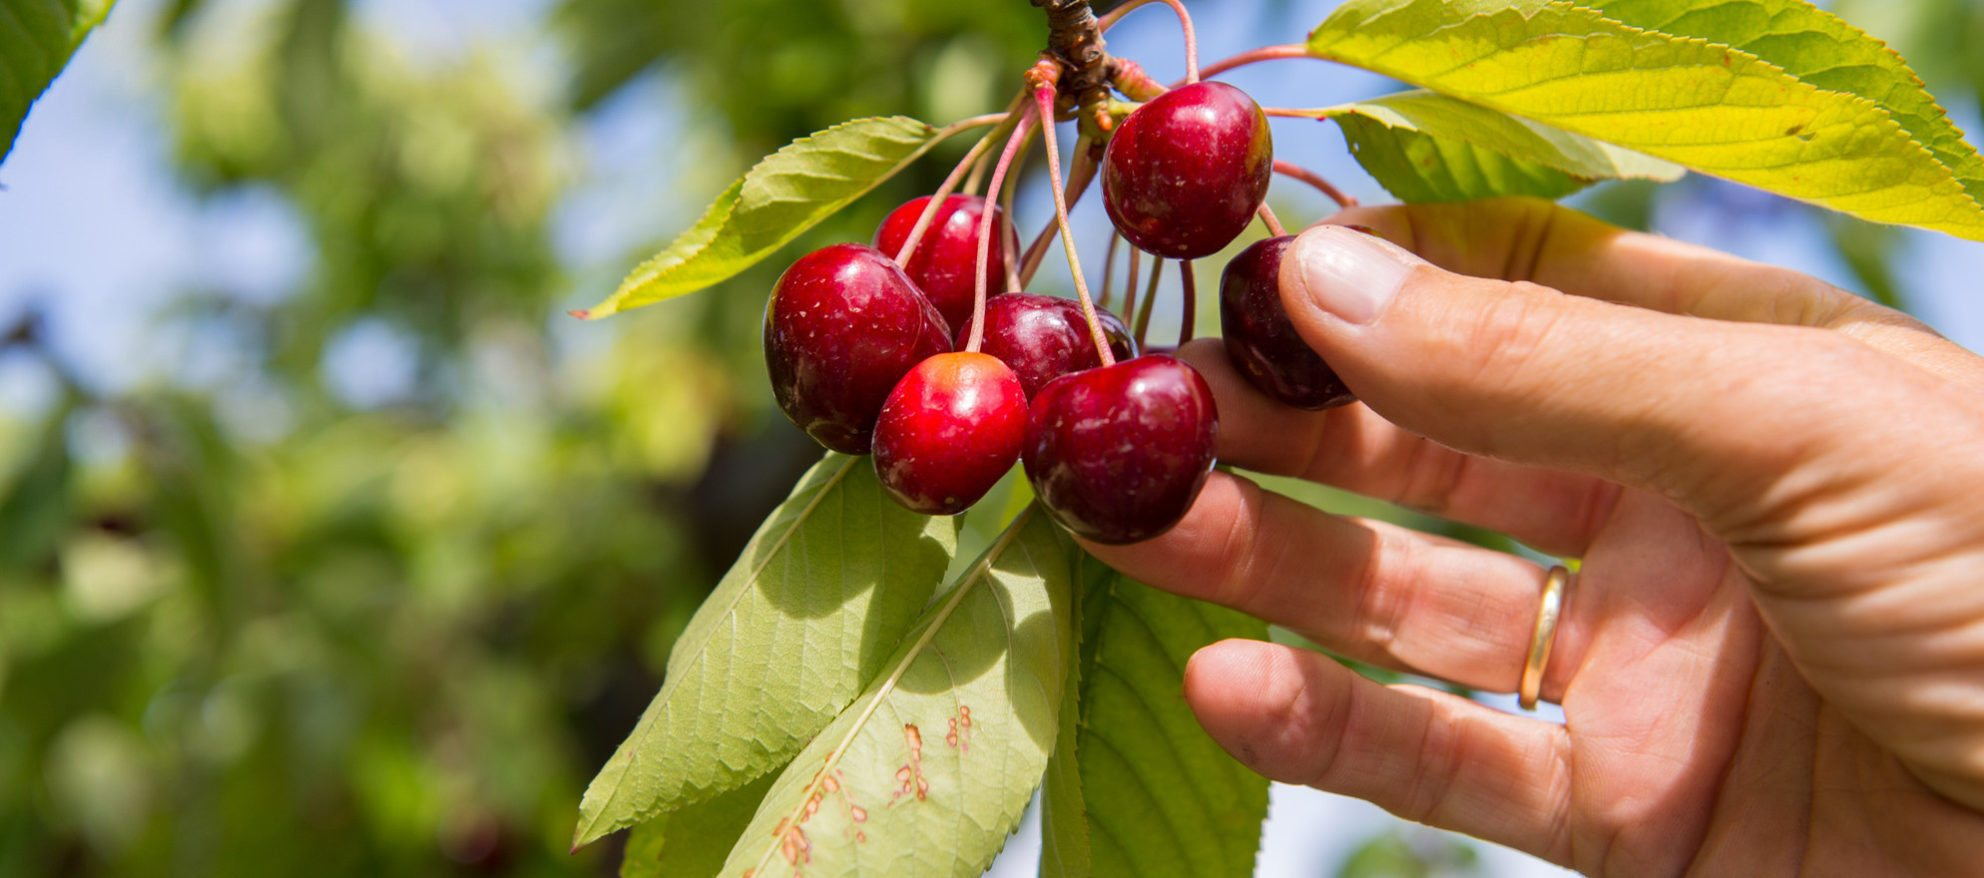
\includegraphics[width=\linewidth]{img/cherry.jpg}
    \end{frame}

    \begin{frame}
        \frametitle{Exemple d'une modele en developpement}
        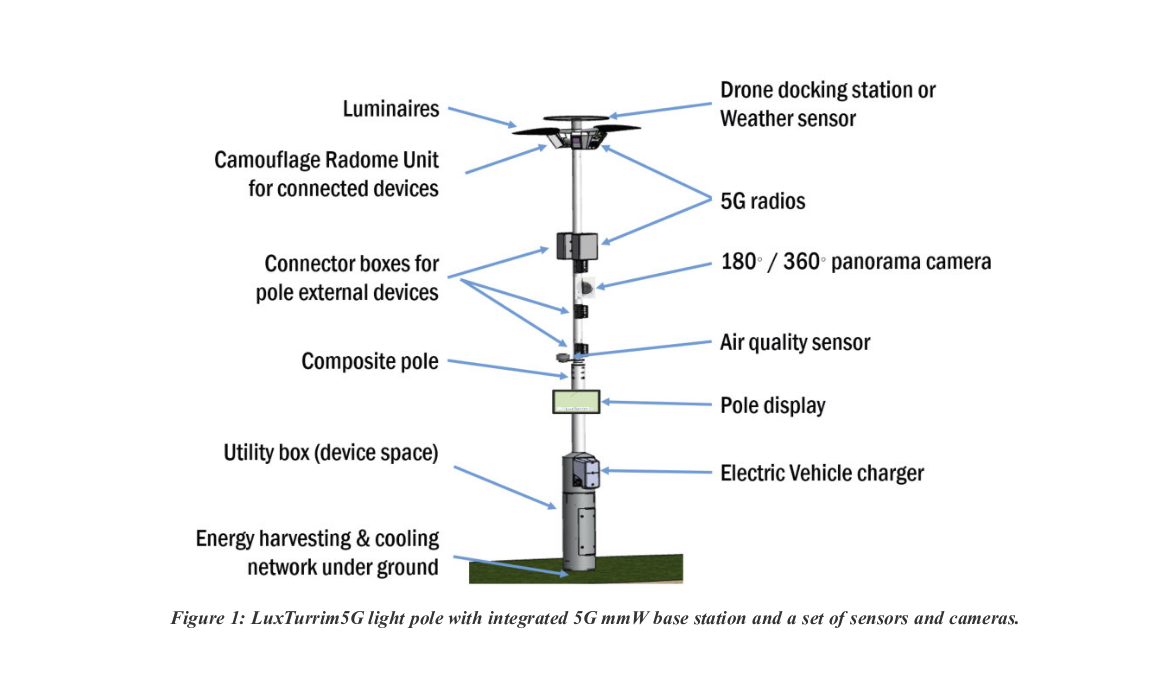
\includegraphics[width=\linewidth]{img/Antenne.png}
    \end{frame}

    \begin{frame}
        \frametitle{Bon pour l'environnement?}
        
\includegraphics[width=\linewidth]{img/green.jpg}
    \end{frame}

    \begin{frame}
        \frametitle{Les applications possibles de la 5G}
        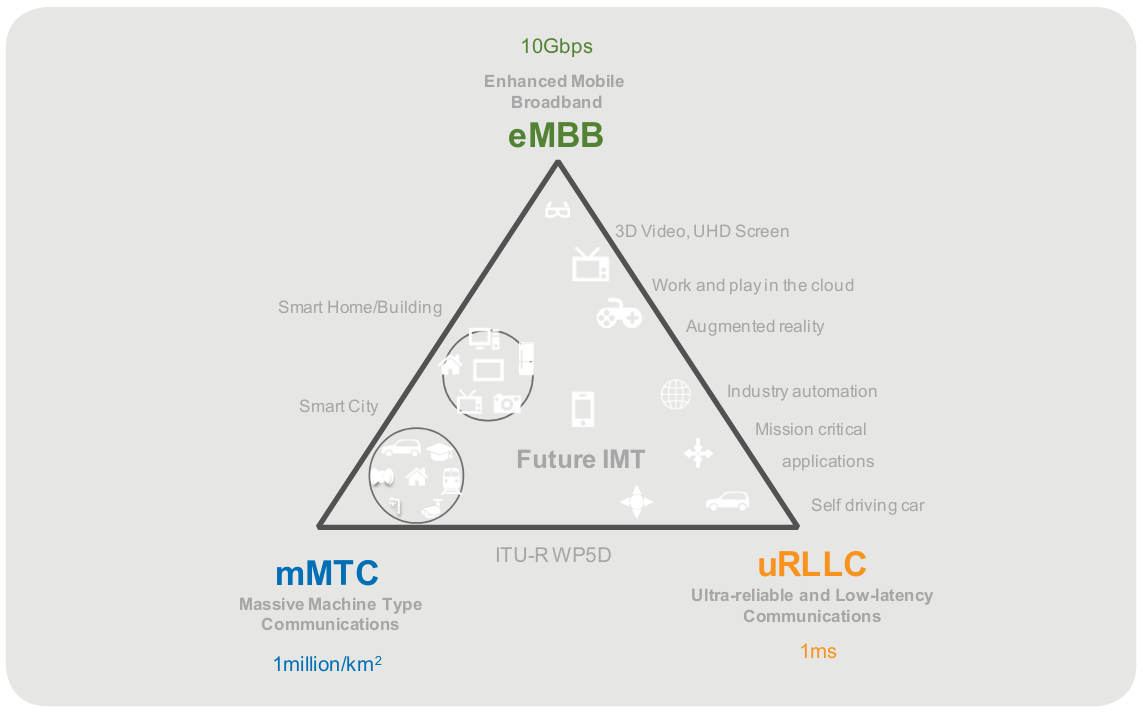
\includegraphics[width=\linewidth]{img/application.png}
    \end{frame}

    \begin{frame}
        \frametitle{}
        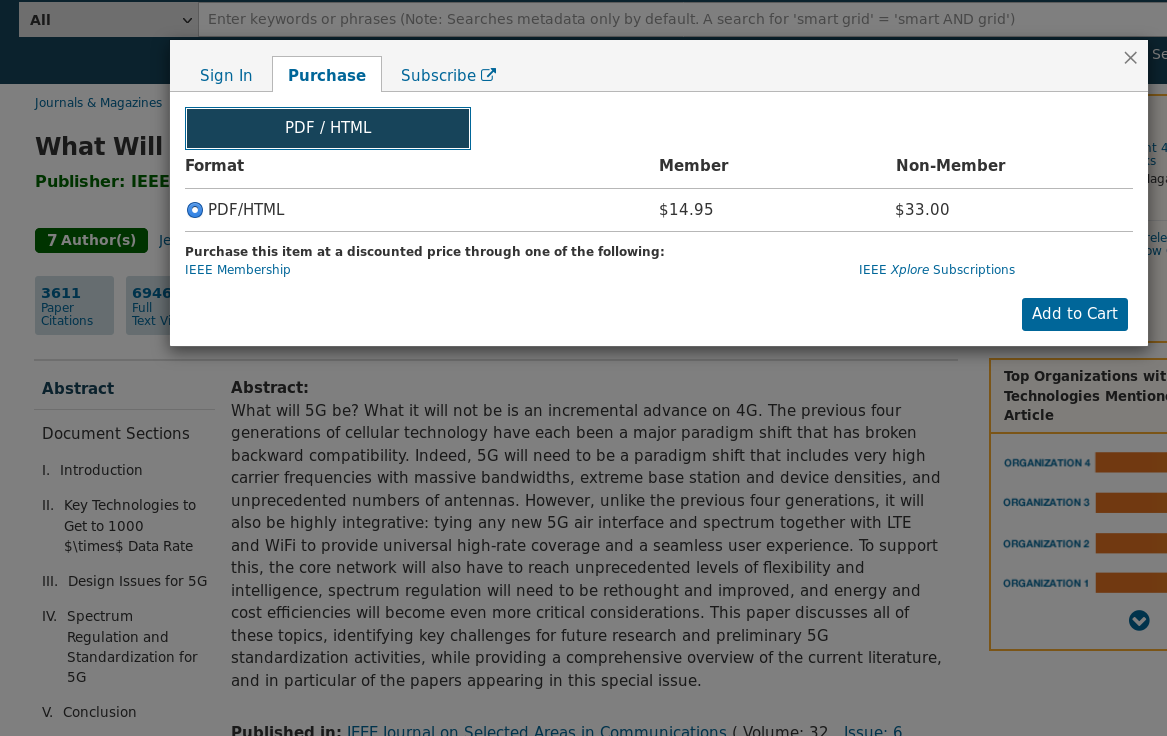
\includegraphics[width=\linewidth]{img/magazine.png}
    \end{frame}

    \begin{frame}
        \frametitle{}
        
\includegraphics[width=\linewidth]{img/sci-hub.jpg}
    \end{frame}

    \begin{frame}
        \frametitle{Sources}
        https://ieeexplore.ieee.org/document/6824752
        https://spectrum.ieee.org/video/telecom/wireless/everything-you-need-to-know-about-5g
        https://ercim-news.ercim.eu/images/stories/EN117/EN117-web.pdf
        https://www.everythingrf.com/community/5g-frequency-bands
        https://www.unwiredinsight.com/2013/lte-mimo
        https://www.blackbox.fr/fr-fr/page/25067/Information/Technique/black-box-explique/Cables-fibre-optique/fibre-optique-monobrin-ou-duplex
        https://www.huawei.com/minisite/hwmbbf16/insights/5G-Nework-Architecture-Whitepaper-en.pdf
    \end{frame}

\end{document}
